\section{Experiments}
\label{sec:experiments}

In this section, we describe the results of our analysis of the \hoot system with the 2008 Twitter dataset used by Sandler and Wallach\cite{sandler09}. This data contains 10,766,525 tweets with 255,833 hash tag references. Additionally, we show the results of experiments using our
prototype to examine the computational overhead of implementing \hoot
over all Twitter traffic.

\subsection{Cover Traffic}

We first show that Twitter groups provide good possibilities for cover
traffic that \hoot can leverage to hide groups seeking plausible
deniability.

In Figure~\ref{fig:hash-dist}, we show the distribution of number of
tweets for each hashtag in the 2008 dataset, ordered by activity level in a log-log scatter
plot. The
distribution appears to follow a typical power law distribution, with a
few very active hashtags and many hashtags with few tweets. A large
cluster of hashtags appear only once in our dataset. 

This distribution shows us that there is a large spectrum of subscriber
anonymity set sizes that can be taken leveraged for \hoot. To get a high
degree of anonymity, the group can choose a plain tag whose short tag
collides with a popular tag. With such a group, the sudden influx of new
followers will not be as suspicious. Some groups may opt
for better plausible deniability by selecting a tag that is only
moderately popular but serves as a believable innocuous interest for
group members.
%gives
%you plausible deniability as there are relatively few tags dominating
%the space at a given time, and thus appear as legitimate interests. If
%there were a more even distribution of tags, then someone observing you
%following a particular tag would have less incentive to ignore suspicion
%that your activities might be objectionable to them. 

\begin{figure*}[t]
\begin{minipage}[b]{0.48\linewidth}
\centering
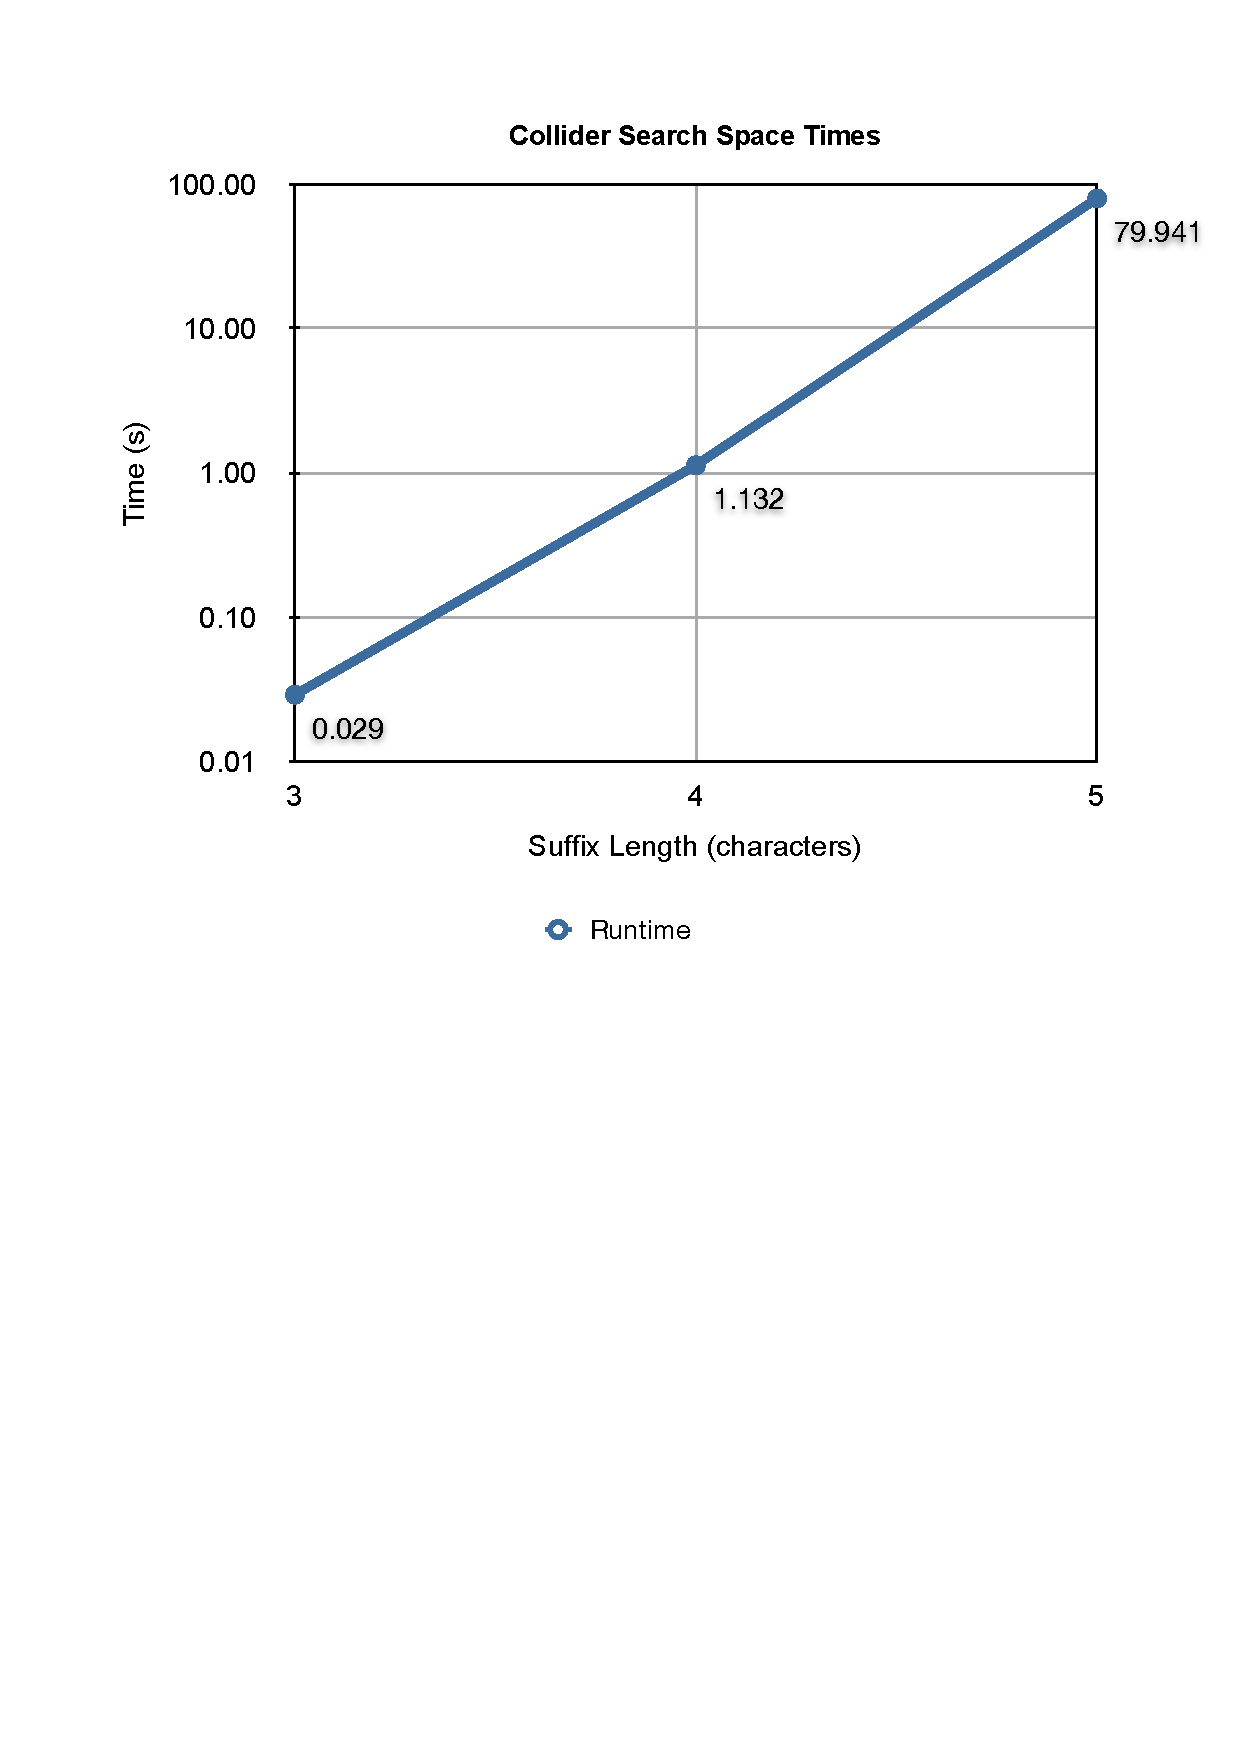
\includegraphics[scale=.5, viewport=0cm 0cm 16.6cm 13.6cm]{collider-times.pdf}
%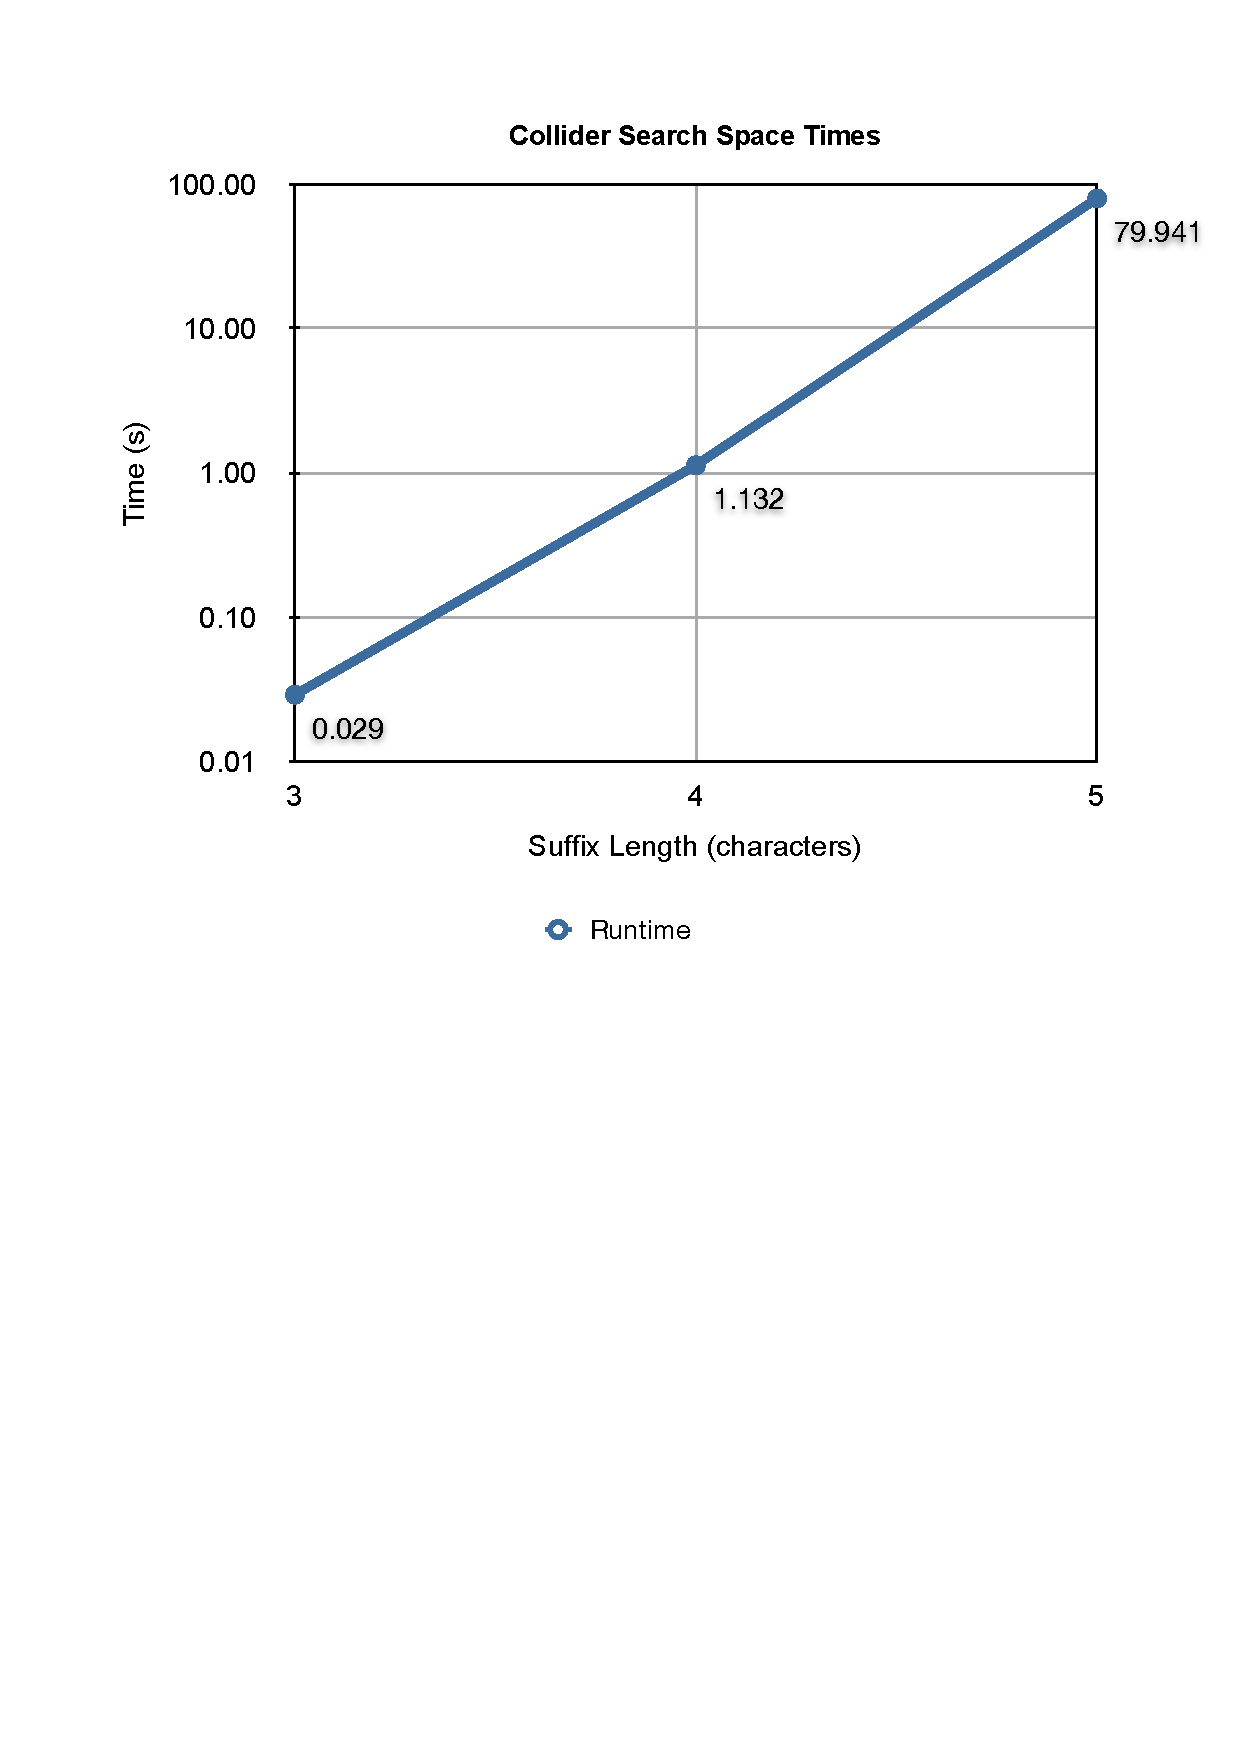
\includegraphics[scale=.5]{collider-times.pdf}
    \caption{Runtime for the collider to search for all matching tags with
  suffixes of length $L=3,4,5$ on a PC with dual quad-core Intel i5
  processors.}\label{fig:collider-times}
\end{minipage}
\hspace{0.5cm}
\begin{minipage}[b]{0.48\linewidth}
\centering
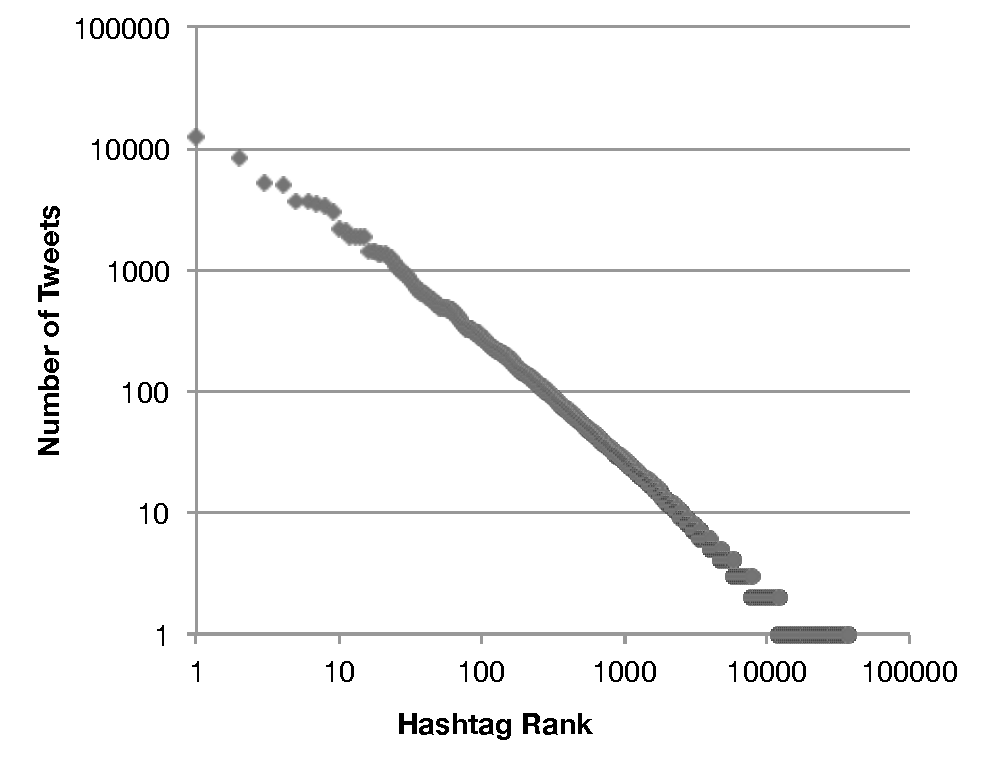
\includegraphics[scale=.5, viewport= 0cm 0cm 16.6cm 12.9cm]{hash-tag-dist.pdf}
%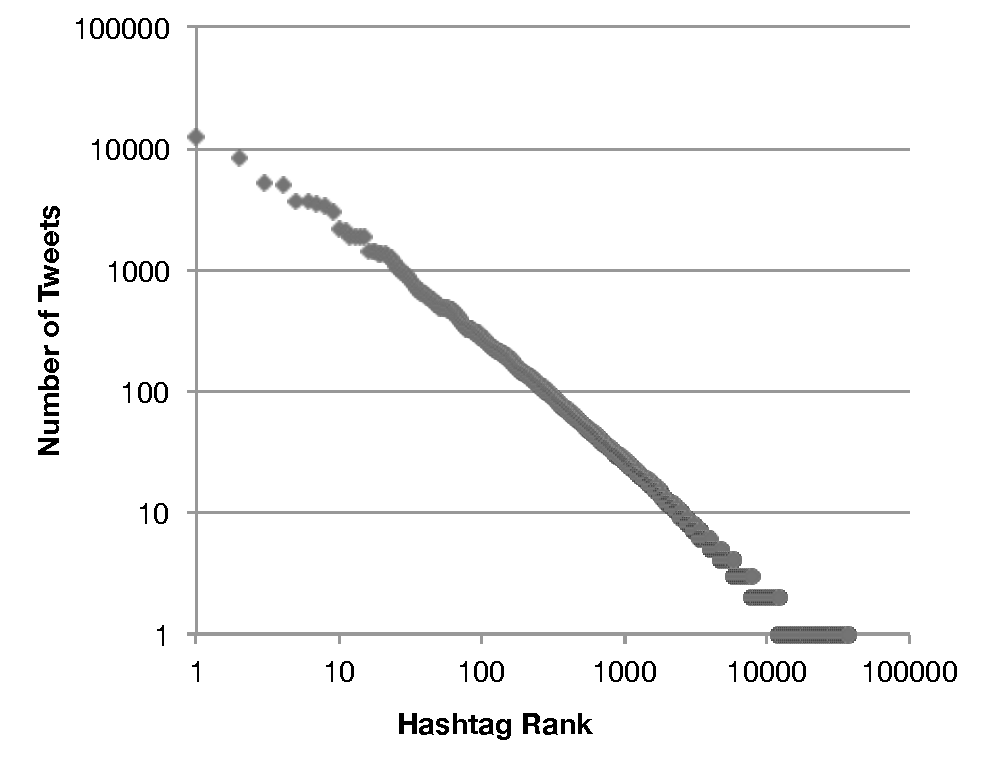
\includegraphics[scale=.5]{hash-tag-dist.pdf}
\caption{2009 Twitter Hashtag activity distribution on a log-log
  scale.\vspace{0.4cm}\label{fig:hash-dist}
}
\end{minipage}
\end{figure*}

\subsection{Collider}
\label{sec:collider}

To explore the feasibility of finding a plain tag that collides with an
existing short tag, we built a tool called the {\em collider} in C and
OpenMP 3.0, using the open source CommonCrypto\footnote{\url{http://www.opensource.apple.com/source/CommonCrypto/}} library provided
by Apple.
The collider takes in a short tag, \textit{T}, a prefix string,
\textit{S}, a suffix length, \textit{L}, an alphabet \textit{A}. It
finds the concatenations of \textit{S} and strings of length \textit{L}
from \textit{A*} such that the truncated hash of the resultant string
matches \textit{T}.

The collider has two modes of operation. In the default mode, he user
specifies the desired number of colliding tags. The collider begins its
scan at a random point in the search space and continues scanning until
the requested number of tags are found. The second mode scans the entire
search space and therefore returns all matching tags for a given prefix
and suffix length.

The search space is of size $|A|^L$. If we wanted to match byte strings,
$|A| = 256$. However, since Twitter operates on characters and not
bytes, we restrict the alphabet to alphanumeric characters, yielding
$|A| = 62$. We note that the search space can be explored in parallel,
which makes the runtime of the collider executing on a system with
\textit{P} processing units $O(\frac{62^L}{P})$.

\begin{figure}
\begin{center}
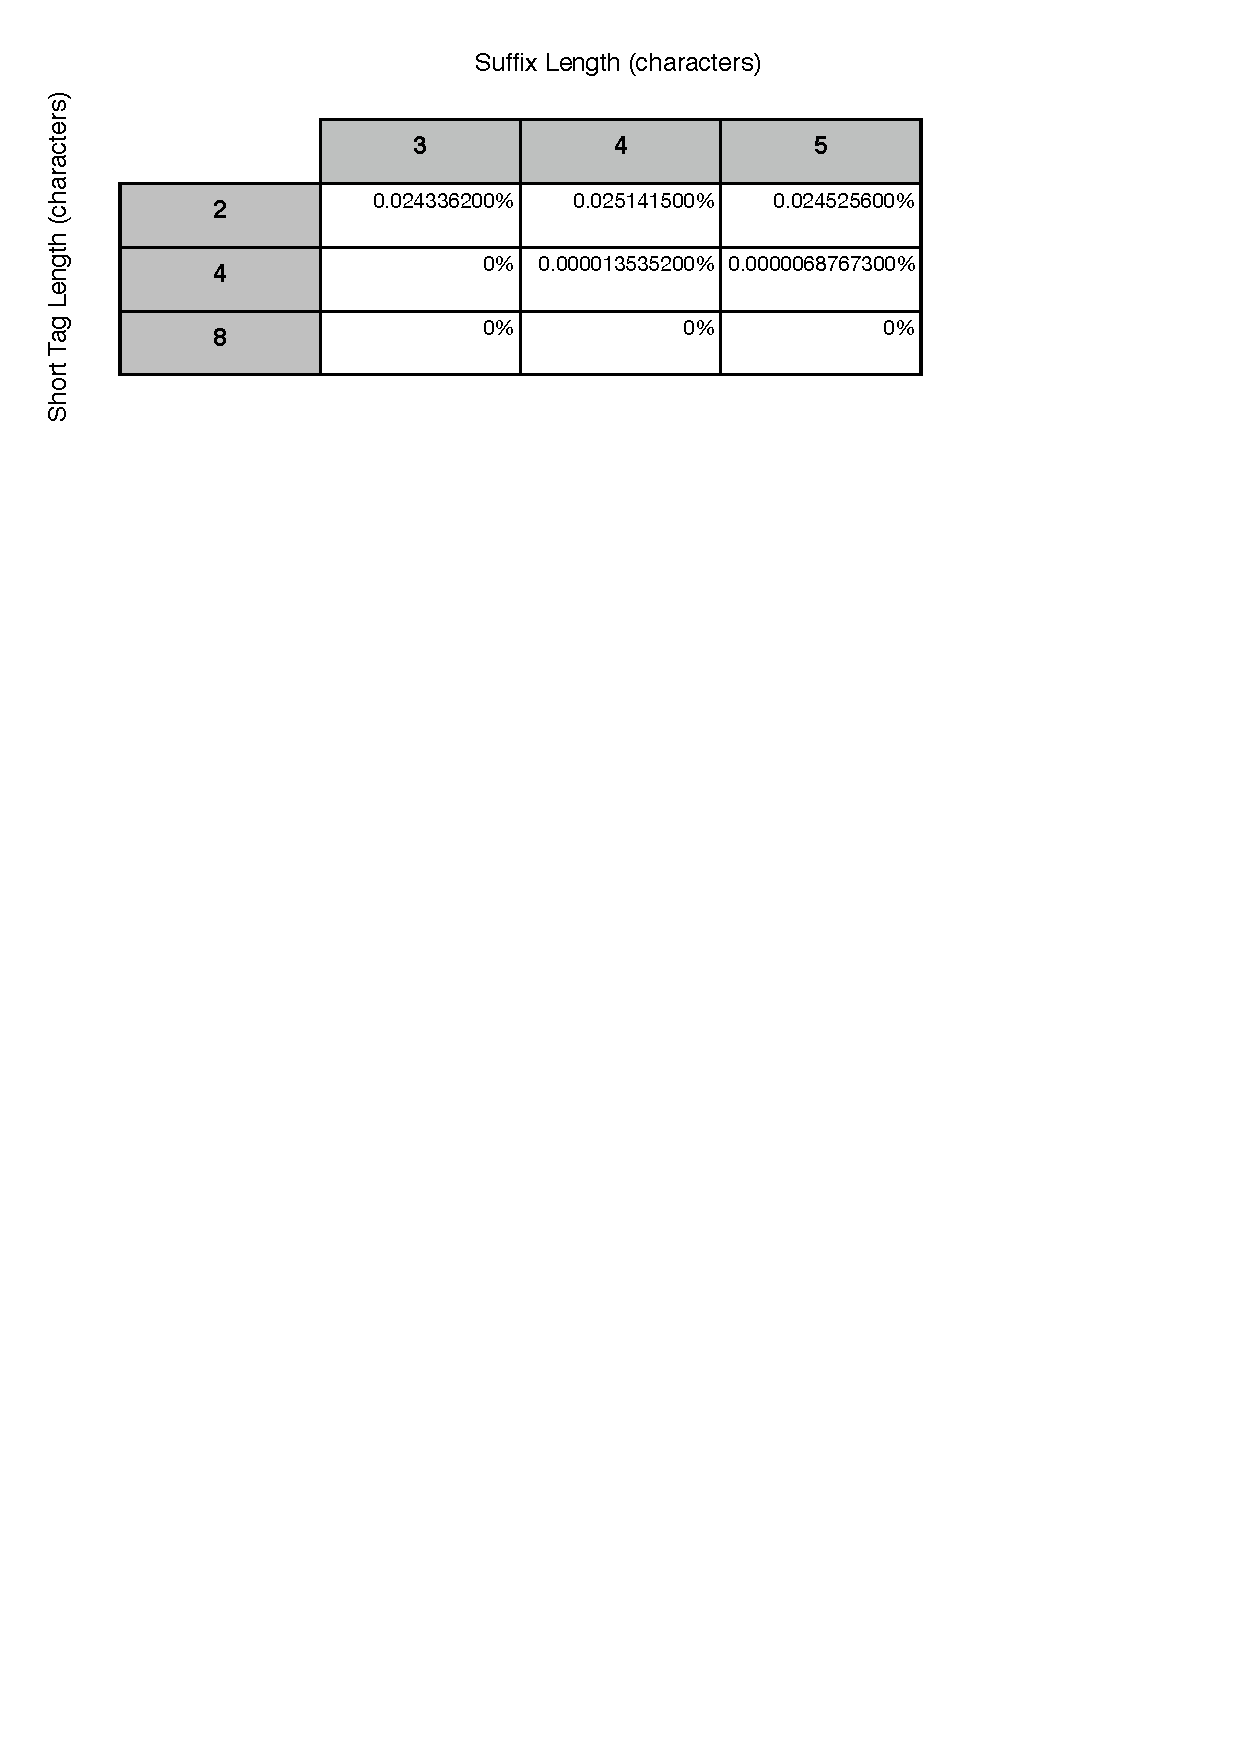
\includegraphics[scale=.5, viewport=0cm 0cm 16.5cm 7.5cm]{collider-hits.pdf}
\caption{Percent of search space that returned hits for an entered short
  tag, with a Prefix of `rice', and given Suffix Length. We used the
  short tags `Ch', `Char', and `CharlieS' for short tags of length two,
  four, and eight, respectively.}\label{fig:collider-hits}
\end{center}
\end{figure}


As expected, the runtime---shown in
Figure~\ref{fig:collider-times}---scales exponentially with \textit{L}.
With our implementation, it is currently infeasible for a single PC to
do an exhaustive search for a suffix length greater than six in a
reasonable amount of time, e.g. less than a day.  \hlfixme{We really
  need to talk about time to find one useful suffix. This story sucks (=
  hoot is unusable!) and you only need one useful suffix in practice.}

%Even if optimizations
%could speed up the calculation, it would likely need to take less than
%an hour to be usable for most groups. On the other hand, finding a
%collision for a short tag is proportional to its size relative to the
%search space.  \hlfixme{FiXme: What about finding one useful suffix?
%  That's the real question...}  \hlfixme{Isn't search time for a single
%  match independent of the search space of the suffix length and
%  dependent on the search space of the short tag length? Or can we not
%  assume even distribution of matching tags? Can I make that argument or
%  am I missing something?}

Another concern is the ability to find colliding tags at all. The
probability $p_{coll}$ of trying $|A|^L$ tags and finding at least one
that has the same short tag as an existing $c$-character tag is given
by:
%
\[p_{coll} = 1-\left(1-\frac{1}{|A|^c}\right)^{|A|^L}.\]
%
For an alphabet of $|A|=62$ glyphs and a short tag length of $c=2$, a
suffix of $L=3$ characters is enough to nearly guarantee at least one
collision. For a short tag length of $c=4$, a suffix of $L=5$ is
required. 
% mkw -- I can't figure out the general formula.
% The 
% \hlfixme{Numerically, on my calculator, I notice that for
%  A=62, L=c will give you prob. 0.643, and L=c+1 gives you very
%  tiny. That's not a coincidence -- find the correspondence.}

To validate this analysis with real tags, we studied the number of
collisions we could find for various values of $c$ and $L$ for a
specific prefix (``rice'') and fixed short tag values. The results,
shown in Figure~\ref{fig:collider-hits}, confirm that short tags of
length four require a suffix of length four or more to find a collision.

Thus recipient anonymity is attainable for short tags of length four or
less, and tied to this is recipient deniability. The more innocuous
traffic that is pulled, the more it seems as if you are truly following
some hot topic, rather than a more clandestine group. An observer
monitoring the tweets you download will be unable to differentiate
someone following a secret group and someone following a popular topic
because members of both groups will pulling all HooTs from each other's
groups.

%how easy it is to collide with another tag. From
%Fig. \ref{fig:collider-hits}, we find that beyond 4 characters, it was
%impossible to find collisions within easily searchable spaces (suffix
%sizes < 6).

%You can only collide with up to 4
%characters in a tag before the search space becomes such that any
%guarantee of collision is trivially small. 
%Furthermore, $62^6$ is the upper bound on the search space for what a
%single computer can reasonably calculate as a suffix to enable a
%collision. Adding one more character to the suffix sends the computation
%into the span of days on a modern computer at time of writing.
%
%However, we also show that tag collision is possible, there are certainly tunab%le degrees of anonymity thanks to the apparent power-log distribution of twitte%r tags already, and finding such a collision is feasibly done on a personal com%puter. \hl{What more to say here?}

\subsection{Performance}

Adoption of \hoot requires that the overhead for encryption and
decryption be reasonable. One path to adoption would have Twitter or
another microblogging service offer \hoot for users seeking group
privacy or censorship resistance. We thus consider computation overhead
in the context of encrypting all Twitter traffic as a worst case. In
March 2011, Twitter stated that the site receives 140 million tweets per
day or 1620 tweets per second on average
(\url{http://blog.twitter.com/2011/03/numbers.html}). They also said
that the maximum tweets per second ever was 6939. These numbers act as
rough upper bounds to the number of Hoots per second the system would
need to keep up with. In all likelihood, the number of encrypted
messages posted would be drastically smaller than regular messages, at
least in the early deployment of \hoot.

\begin{table}
\caption{Average Hoots Per Second for Encryption and Decryption
\label{tab:hps}
}
\begin{center}
    \begin{tabular}{ l  l }
	\hline
	Action & Average hoots per second \\ \hline
	Encryption & 3610 \\
	Decryption & 15590 \\ \hline
%	Encryption & 3614.531 \\
%	Decryption & 15587.328 \\ \hline
    \end{tabular}
\end{center}
\end{table}

To study the amount of computation required to support \hoot over
Twitter, we modified our Python script to perform the encryption process 
500,000 times running on a MacBook
Air with a 1.86GHz Intel Core 2 Duo and 4GB Ram using Base64 encoding. We 
also independently performed the decryption process 500,000 times. We 
record how long each process took and divide by 500,000. In
Table~\ref{tab:hps}, we see the result of this experiment. The amount of
computation for encryption is negligible for Twitter: the average load
can be handled by one laptop. A Twitter server could easily encrypt the
entire Twitter feed as the messages were posted. To handle peak usage
like the 6939 tweets per second Twitter observed, a variety of
optimizations could be made and, if necessary, the server could be a
more powerful machine with more processors.

The decryption rate is important to clients, since clients will need to
search through hoots with colliding hashtags and decrypt the session
keys for each one to see if it decrypts correctly. Note that, with a
simple fixed constant string prepended to the keys, the client can
quickly verify whether the message was encrypted using $k_{tag}$ or if
another group's key was used. Since our process can decrypt Hoots almost
five times faster than it encrypts them, even clients with limited
computing power can keep up with the entire Twitter feed. In practice,
clients would only need to decrypt hoots that share the same short tag,
which should be a small fraction of this cost even for very active
groups.

%A client may not trust Twitter to do the decryption since that involves
%sharing the plain tag with Twitter, so a client would decrypt the
%message on their machine. Almost every client will not have a datacenter
%of computers for decryption, but 
%adopted with little engineering effort.

%\hl{Should experiments have a wrap up paragraph?}

%\hlfxnote{mkw -- I don't think so. We'll cover more ground in the discussion.}

